% !TEX root = thesis.tex

%%
%%
%% Method chapter
%%
%%

In this chapter, we describe the methods used to examine the statistical performance of the \gls{dkd}.
The basic unit is the \textit{experiment},
a set of simulations run with the same initial setup with the same measurements taken.
Each experiment is run with a fixed set of parameters, described below in \Cref{tab:experimental_parameters}.
We then run a set of experiments,
varying one parameter at a time, or in some cases two parameters in tandem,
in order to observe the effect of this parameter on the accuracy of the \gls{dkd}.

\begin{table}[htbp]
    \centering
    \begin{tabular}{ll}
        \toprule
        Parameter name & Description \\
        \midrule
        x1.min & Minimum value of the study area in the horizontal ($X_1$) direction \\
        x1.max & Maximum value of the study area in the horizontal ($X_1$) direction  \\
        x2.min & Minimum value of the study area in the vertical ($X_2$) direction \\
        x2.max & Maximum value of the study area in the vertical ($X_2$) direction \\
        grid.by & Space between grid points in the study area \\
        buffer & Buffer around outside of study area \\
        N.p & Size of population \\
        EN.i & Expected number of incidents per simulation \\
        c1 & (optional) $x_1$ coordinate of the population peak \\
        c2 & (optional) $x_2$ coordinate of the population peak \\
        sigma1 & (optional) $x_1$ standard deviation of the population peak \\
        sigma2 & (optional) $x_2$ standard deviation of the population peak \\
        rho & (optional) Correlation coefficient of $x_1$ and $x_2$ \\
        bandwidths & List of bandwidths for evaluating the Oracle \\
        incident\textunderscore rate & Risk function for generating incidents from population \\
        \bottomrule
    \end{tabular}
    \caption{Experimental parameters}
    \label{tab:experimental_parameters}
\end{table}

\setpath{./results/unif_500_1.0_1h/}
\begin{figure}[htbp]
        \centering
    \begin{subfigure}[t]{0.33\textwidth}
    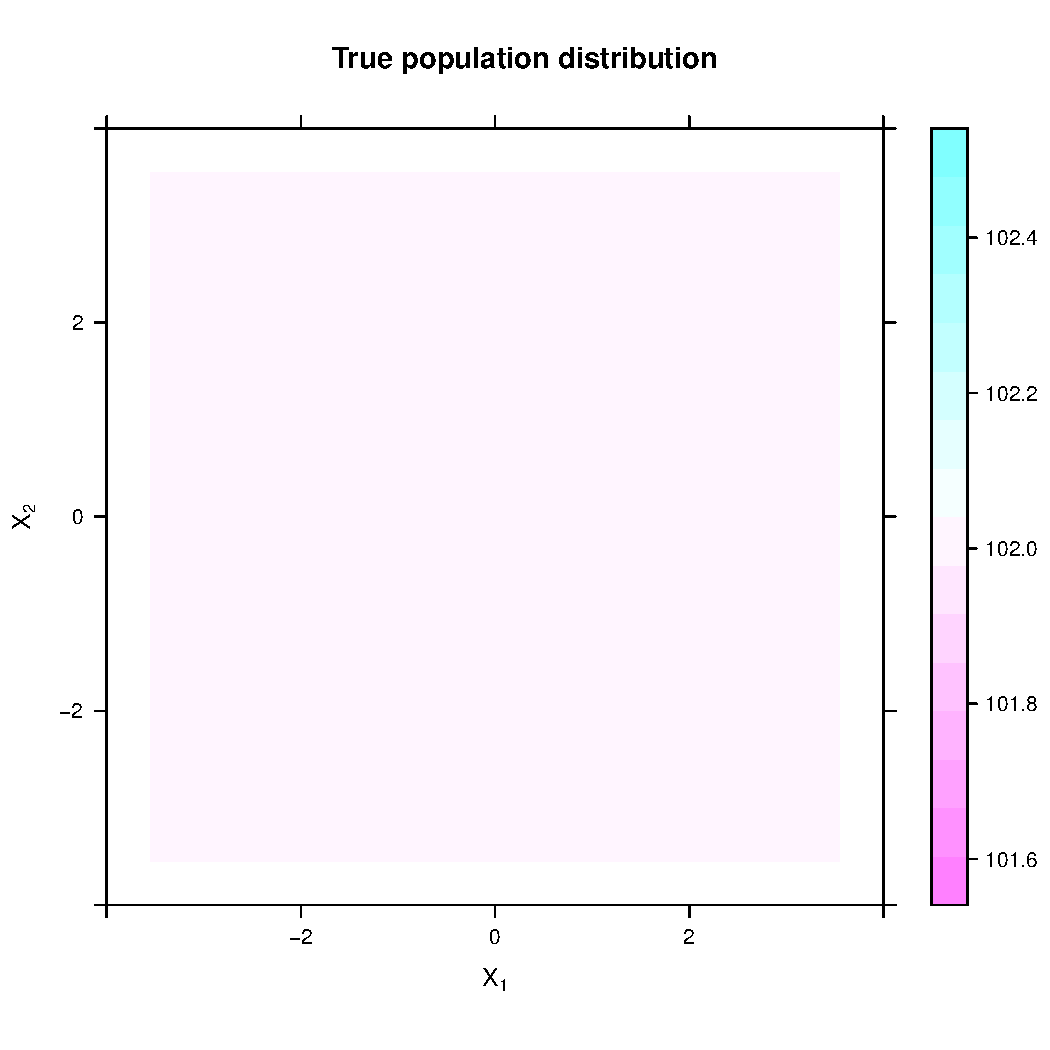
\includegraphics[width=\textwidth]{output/population-heatmap}
    \subcaption{Population distribution}
    \end{subfigure}
    \begin{subfigure}[t]{0.33\textwidth}
    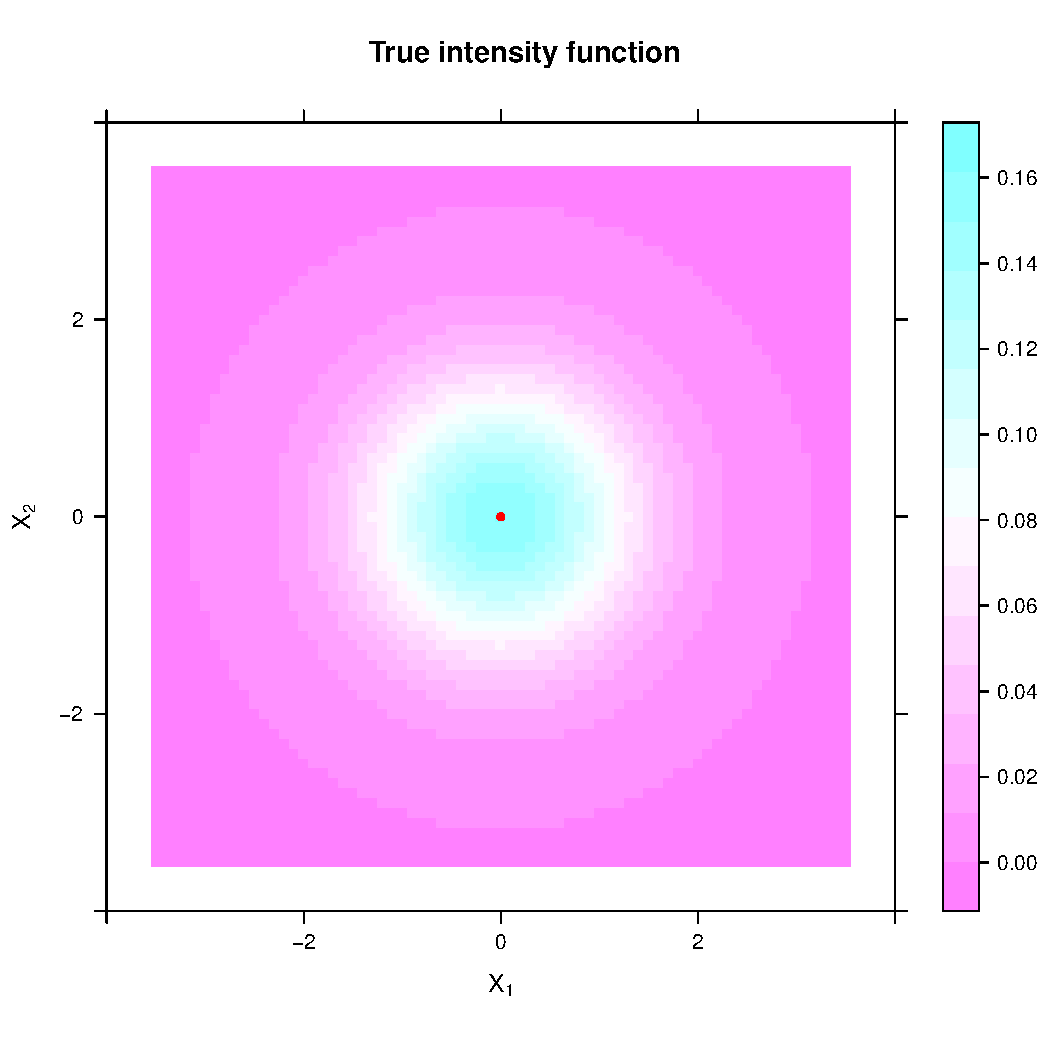
\includegraphics[width=\textwidth]{output/true_intensity_heatmap}
    \subcaption{True risk function}
    \end{subfigure}%
    \begin{subfigure}[t]{0.32\textwidth}
    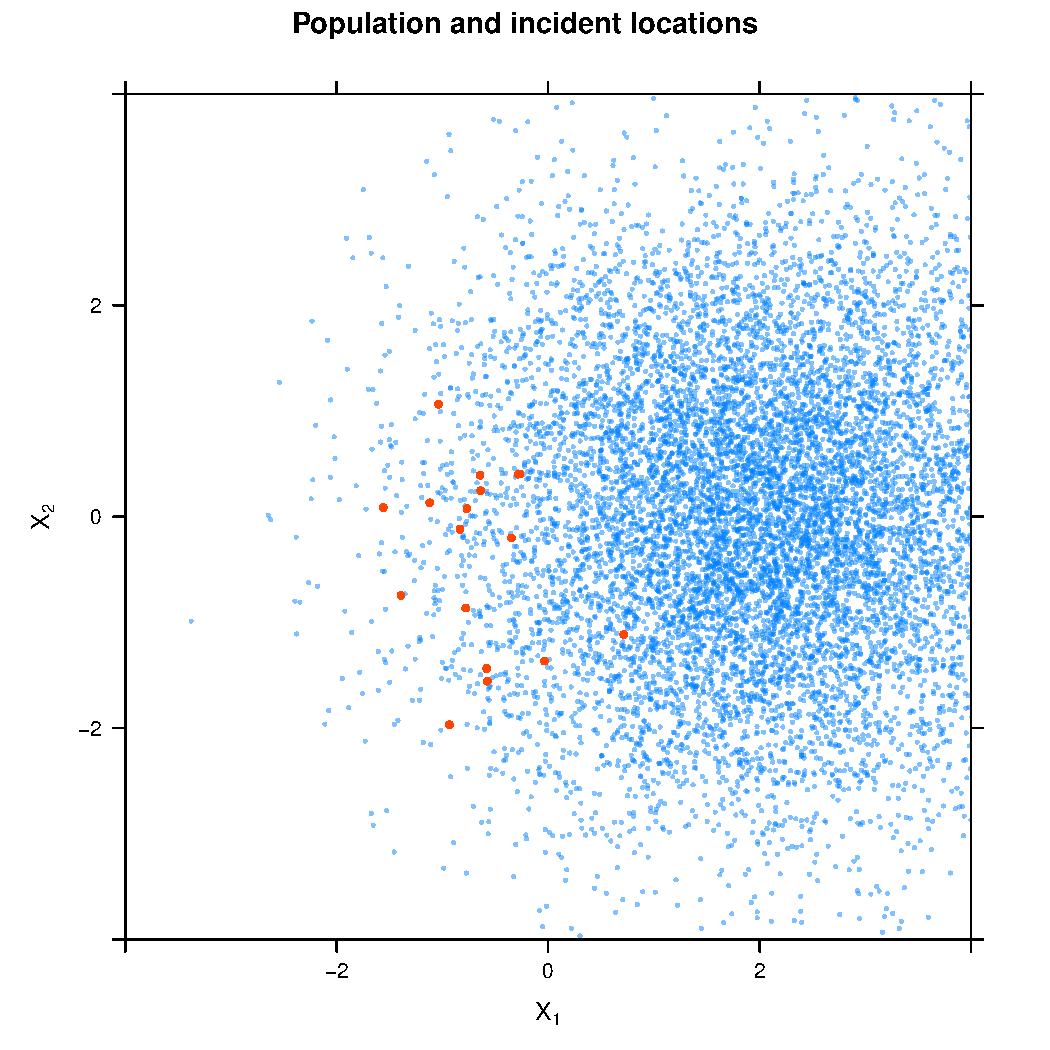
\includegraphics[width=\textwidth]{output/population_and_incidents_scatter}
    \subcaption{Population points (gray) with incidents (black)}
    \end{subfigure}%

    \caption[]{Population distribution (a), true risk function (b), and sample population with incidents (c) for uniform population of 10,000, single-peak risk of \gls{spread} 1.0 and \gls{factor} 500}
    \label{fig:method:distributions:unif_500_1.0_1h}    
\end{figure}
\setpath{}
The \gls{dkd} method can be used to estimate a \textit{rate},
in cases where a set of incident locations and a corresponding set of population locations are available.
by separately computing the \gls{kernel intensity estimator}
\Cref{fig:method:distributions:unif_500_1.0_1h} shows an example a uniform population distribution function in (a),
and a true, single-peak risk function in (b),
with the lighter colored areas having higher risk.
\Cref{fig:method:distributions:unif_500_1.0_1h}(c) shows the population as lightly colored dots,
and the incidents as darker triangles.
Some real-life examples of where the \gls{dkd} can be used include disease incidence rates,
insurance claim rates,
where the population would be insured homes and the incidents would be claims,
and product sales rates where the population would be people who were targeted with a promotion and the incidents would be sales.
Statistically these are modeled as \glspl{spp},
in particular as inhomogeneous Poisson processes
as defined in \Cref{defn:inhomogenouspoissonprocess} in \Cref{sec:theory:spatial_point_processes}.

The rest of this chapter is organized as follows:
\Cref{sec:method:computing} describes how an estimate \gls{lambda_hat} for a risk function \gls{lambda} in the plane is estimated using the \gls{dkd}.
In \Cref{sec:method:accuracy}, we define the measures of accuracy we use to evaluate the \gls{dkd}.
\Cref{sec:method:data generation} describes how sample data is generated.
Our use of \gls{cv} for bandwidth selection is discussed in  \Cref{sec:method:cross-validation}.
\Cref{sec:method:experiment_structure} describes the steps of each experiment, together with the measurements taken.
Finally, in \Cref{sec:method:combining_experiments}, we describe how the effect of different variables are studied by combining several experiments and comparing their results.

%%%%%%%%%%%%%%%%%%%%%%%%%%%%%%%%%%%%%%%%%%%%%%%%%%%%%%%%%%%%%%%%%%%%%%%%%%%%%
%
% Section: Data generation process
%
%%%%%%%%%%%%%%%%%%%%%%%%%%%%%%%%%%%%%%%%%%%%%%%%%%%%%%%%%%%%%%%%%%%%%%%%%%%%%
\section{Data generation process}
\label{sec:method:data generation}

We generate data for each experiment as follows.
Before we begin, we set the random number seed to a fixed value for all experiments.
The first step is to generate a population.
We choose a distribution function $f_p$ over \gls{W},
and scale it to obtain the population intensity function \gls{lambda_P} of a \gls{spp} \gls{Lambda}
with an expected number of points the same as our chosen population size.
For example,
start with a 2-dimensional Gaussian function with standard deviation 1 in both directions and no correlation.
This function has expected value 1, so if we multiply it by 10,000,
the resulting product will be an intensity function \gls{lambda_P} will have expected value 10,000.
This function,
when used as an intensity,
will generate on average 10,000 people,
concentrated around the center $(0,0)$.
However, in a given realization,
the actual population size may not be exactly what we have chosen.

The actual process of generation is as follows.
We generate points $\xvec$ in \gls{W} from the \textit{uniform} random vector $(X_1,X_2)$,
and keep them with probability \gls{lambda_P}$\xvec$.
This gives us our population \gls{P} which we use throughout the experiment.
In this way,
if \gls{lambda_P}$\xvec$ has twice the value of \gls{lambda_P}$(y_1, y_2)$ for two points $\xvec$ and $(y_1, y_2)$ in \gls{W},
then we expect to see about twice as many points around $\xvec$ than around $(y_1, y_2)$ in \gls{P}.

Once we have a fixed population, we have to decide which members of the population constitute the incidents.
The process to generate the incidents is similar to that of the population.
We create an incident intensity function \gls{lambda_I} of a \gls{spp} for incidents.
We then take the points $\xvec \in \gls{P}$ and keep each one with probability \gls{lambda_I}$\xvec$.
This gives us our set of incidents \gls{I}.
Once again, when \gls{I}$\xvec$ is higher than \gls{I}$(y_1, y_2)$,
then the probability of $\xvec \in \gls{I}$ is correspondingly higher than that of $(y_1, y_2)$.

%%%%%%%%%%%%%%%%%%%%%%%%%%%%%%%%%%%%%%%%%%%%%%%%%%%%%%%%%%%%%%%%%%%%%%%%%%%%%%
%%
%% Section: computing the dkd
%%
%%%%%%%%%%%%%%%%%%%%%%%%%%%%%%%%%%%%%%%%%%%%%%%%%%%%%%%%%%%%%%%%%%%%%%%%%%%%%%
\section{Computing the DKD}
\label{sec:method:computing}

The \gls{dkd} is computed over the study area \gls{W} as the ratio of two positive-valued functions.
Recall from \Cref{defn:studyarea} that \gls{W} is the region in the plane where we make observations.
At any given point $\xvec$ in the plane, we can compute \gls{lambda_I}$\xvec$, the \gls{factor} at that point.
We call \gls{lambda_I}$\xvec$ the \textit{incident intensity} at $\xvec$.
Next, at the same point, we can compute \gls{lambda_P}$\xvec$, the \textit{population intensity} at $\xvec$.
Ideally, we would know how to compute these functions exactly, and we would then compute $\lambda\xvec$ the risk,
or probability of an incident at $\xvec$ with the ratio:
\begin{equation}
    \lambda\xvec = \frac{\gls{lambda_I}\xvec}{\gls{lambda_P}\xvec}.
\end{equation}

In practice, these functions are not known and we cannot compute \gls{lambda_I}$\xvec$ and \gls{lambda_P}$\xvec$ exactly, 
so we estimate them from observational data,
using a \gls{kernel intensity estimator} as described in \Cref{eq:lambda_hat},
but with separate bandwidths $h_1$, $h_2$.
As noted in \Cref{sec:theory:kernelestimation},
we use the biweight or quartic kernel with formula \Cref{eq:biweightkernel2d}.

For simplicity of computation, we do not account for edge effects.


%%%%%%%%%%%%%%%%%%%%%%%%%%%%%%%%%%%%%%%%%%%%%%%%%%%%%%%%%%%%%%%%%%%%%%%%%%%%%%
%%
%% Section: accuracy measures
%%
%%%%%%%%%%%%%%%%%%%%%%%%%%%%%%%%%%%%%%%%%%%%%%%%%%%%%%%%%%%%%%%%%%%%%%%%%%%%%%
\section{Measuring the accuracy of the DKD}
\label{sec:method:accuracy}

In order to describe the accuracy of the \gls{dkd} as a method of estimating the true risk function $\lambda$,
we use several accuracy measures.

%%%%%%%%%%%%%%%%%%%%%%%%%%%%%%%%%%%%%%%%%%%%%%%%%%%%%%%%%%%%%%%%%%%%%%%%%%%%%%
%% Subsection: MISE
%%%%%%%%%%%%%%%%%%%%%%%%%%%%%%%%%%%%%%%%%%%%%%%%%%%%%%%%%%%%%%%%%%%%%%%%%%%%%%
\subsection{MISE}
\label{subsec:method:mise}

\Gls{mise} is a measure of the expected squared difference between an estimated risk function \gls{lambda_hat},
computed using the \gls{dkd}, and the true risk function \gls{lambda}.
\Gls{mise} allows for additional analysis by being broken down into the mean integrated squared bias and mean integrated variance.
It can also be easily approximated by cross-validation error.

For any given data sample, we can use the \gls{dkd} to compute the estimated risk function \gls{lambda_hat}.
We wish to compute the \gls{mise} as described in \Cref{eq:mise}.
However, it is computationally impractical to compute this integral.
Instead,
we run $M$ monte carlo simulations and approximate the \gls{mise} by taking the empirical average of the \glspl{ise}.

\begin{equation}
    \label{eq:mise_tilde}
    \widetilde{\mbox{MISE}} = \frac{1}{M} \sum_{i=1}^{M} \mbox{ISE}(\hat{\lambda_I})
\end{equation}

In many of our analyses, we compare the accuracy of several experiments.
\gls{mise} is computed from the \gls{ise},
and \gls{ise} as computed using \Cref{eq:ise}.
For any $\gls{lambda_hat} := \gls{lambda_hat}\dotdot$ we have $\gls{lambda_hat} = \gls{mu} \hat f $,
and correspondingly $ \mbox{\gls{mise}}(\gls{lambda_hat}) = \gls{mu}^2 \mbox{\gls{mise}}(\hat f) $.

We observe that \gls{mise} will naturally increase with \gls{mu} when computed in an absolute sense.
We provide two variations of the \gls{mise} that compensate for this.
First, we compute \gls{rmise} by dividing $\gls{lambda_hat}\xvec$ by $\gls{lambda}\xvec$ at every point $x_1, x_2$ in the evaluation grid, and computing
\begin{equation}
\label{eq:rmise}
    \mbox{\gls{rmise}}(\gls{lambda_hat}) = 
        \mbox{\gls{mise}}(\gls{relative_lambda_hat}) \\
\end{equation}
where
\begin{equation}
\label{eq:relative_lambda_hat}
    \gls{relative_lambda_hat}\xvec = 
        \frac{\gls{lambda_hat}\xvec}{\gls{lambda}\xvec}
        \text{.}
\end{equation}

We also \textit{normalize} the \gls{mise} by dividing by $\gls{mu}^2$,
which we call \gls{nmise}:
\begin{equation}
\label{eq:nmise}
    \mbox{\gls{nmise}}(\gls{lambda_hat}) = 
        \frac{1}{\gls{mu}^2} \mbox{\gls{mise}}(\gls{lambda_hat}) \text{.}
\end{equation}

Often we are comparing the results of several experiments.
Sometimes, the \gls{factor} \gls{mu} has different values in each of those experiments.
In such a case, it is more informative to compare the accuracy of two experiments using \gls{nmise} and \gls{rmise} than using \gls{mise},
since the \gls{mise} describes the absolute accuracy of the estimate and its value is highly dependent on the scale of the true intensity \gls{lambda}.

%%%%%%%%%%%%%%%%%%%%%%%%%%%%%%%%%%%%%%%%%%%%%%%%%%%%%%%%%%%%%%%%%%%%%%%%%%%%%%
%% Subsection: MIAE
%%%%%%%%%%%%%%%%%%%%%%%%%%%%%%%%%%%%%%%%%%%%%%%%%%%%%%%%%%%%%%%%%%%%%%%%%%%%%%
\subsection{MIAE}
\label{subsec:method:miae}

\Gls{miae} is a measure of the expected absolute difference between an estimated risk function \gls{lambda_hat},
computed using the \gls{dkd}, and the true risk function \gls{lambda}.
\Gls{miae} differs from \gls{mise} by on the one hand providing a more intuitive comparison,
since we are comparing the absolute difference instead of the squared difference.
On the other hand, it lacks some of the nice mathematical properties of the \gls{mise}.

As we did in \autoref{subsec:method:mise}, for any given data sample we use the \gls{dkd} to compute the estimated risk function \gls{lambda_hat}.
We then integrate the absolute value of the error in the estimate over the plane to obtain the \gls{ise}.

\begin{equation}
    \mbox{IAE}(\hat{\lambda}) = 
        \iintW{
            \left| \hat{\lambda}\xvec - \lambda\xvec \right|
        }
\end{equation}

We can then compute the expected value of the \gls{ise} to obtain the \gls{mise}.

\begin{equation}
    \mbox{MIAE} = \E [\mbox{IAE}(\hat{\lambda})]
\end{equation}

As above, we run $M$ monte carlo simulations,
and approximate the \gls{miae} by taking the empirical average of the \glspl{iae}.

\begin{equation}
    \widetilde{\mbox{MIAE}} = \frac{1}{M} \sum_{i=1}^{M} \mbox{IAE}(\hat{\lambda_I})
\end{equation}

As with \gls{mise}, we need to compare experiments with different values of \gls{mu}.
The analogous definitions are \gls{rmiae} and \gls{nmiae}, as defined below.

\begin{equation}
\label{eq:rmiae}
    \mbox{\gls{rmiae}} = 
        \mbox{\gls{miae}}(\gls{relative_lambda_hat}) \\
\end{equation}

where \gls{relative_lambda_hat} is defined above in \Cref{eq:relative_lambda_hat},
and

\begin{equation}
\label{eq:nmiae}
    \mbox{\gls{nmiae}} = 
        \frac{1}{\gls{mu}} \mbox{\gls{miae}}(\gls{lambda_hat}) \text{.}
\end{equation}


%%%%%%%%%%%%%%%%%%%%%%%%%%%%%%%%%%%%%%%%%%%%%%%%%%%%%%%%%%%%%%%%%%%%%%%%%%%%%%
%% Subsection: Max error
%%%%%%%%%%%%%%%%%%%%%%%%%%%%%%%%%%%%%%%%%%%%%%%%%%%%%%%%%%%%%%%%%%%%%%%%%%%%%%
\subsection{Supremum error}
\label{subsec:method:sup_error}

Whereas the previous two measures of accuracy describe how much the estimated intensity deviates from the truth over the whole plane,
the \gls{supremum error} looks at the worst case.
We define the \gls{supremum error} as follows:

\begin{equation}
    \mbox{supremum error}(\gls{lambda_hat}) = \sup_{\xvec \in \gls{W}}
        {\left|
            \gls{lambda_hat}\xvec - \lambda\xvec
        \right|}
\end{equation}

As in the previous accuracy measures, we run $M$ monte carlo simulations, and approximate the \mbox{supremum error}, by taking the empirical average of the supremum error of the estimates.

\begin{equation}
    \widetilde{\mbox{\gls{supremum error}}} = \frac{1}{M} \sum_{i=1}^{M} \mbox{supremum error}(\hat{\lambda_I})
\end{equation}

Furthermore, we need to compare experiments with different values of \gls{mu}.
The analogous definitions are \gls{relative supremum error} and \gls{normalized supremum error}, as defined below.

\begin{equation}
\label{eq:relative_supremum_error}
    \mbox{\gls{relative supremum error}}(\gls{lambda_hat}) = 
        \frac{1}{\lambda_{max}} \mbox{\gls{supremum error}}(\gls{lambda_hat}) \\
\end{equation}

where
\begin{equation}
\label{eq:lambda_max}
    \lambda_{max} = \sup_{\xvec \in \gls{W}}{\gls{lambda}\xvec} \text{.}
\end{equation}

\begin{equation}
\label{eq:normalized_supremum_error}
    \mbox{\gls{normalized supremum error}}(\gls{lambda_hat}) = 
        \frac{1}{\gls{mu}} \mbox{\gls{supremum error}}(\gls{lambda_hat}) \text{.}
\end{equation}

%%%%%%%%%%%%%%%%%%%%%%%%%%%%%%%%%%%%%%%%%%%%%%%%%%%%%%%%%%%%%%%%%%%%%%%%%%%%%%
%% Subsection: Peak bias and drift
%%%%%%%%%%%%%%%%%%%%%%%%%%%%%%%%%%%%%%%%%%%%%%%%%%%%%%%%%%%%%%%%%%%%%%%%%%%%%%
\subsection{Peak bias and peak drift}
\label{subsec:method:peak_bias}

The next two accuracy measures compare the estimated risk function's accuracy in estimating the peak.
By estimating the peak,
our goal is to learn the location of the source of observed incidents,
and also its strength.
In order to define them,
we first define the estimated peak,
which is computed as follows,
suggested by \citet{parzen1961mathematical}.
We first compute the \gls{dkd} estimate \gls{lambda_hat} as the estimate of the true rate.
Recall that we evaluate the \gls{lambda_hat} on a fixed, finite grid of points $G \subset W$.
Then,
we evaluate \gls{lambda_hat}\xvec on each of the points in $\xvec \in G$, and take the maximum.
This gives us the location and value of the peak of the \gls{dkd}.
\begin{equation}
    \widetilde{\mbox{peak}} = (p_1, p_2) \in G \|%
        \xvec \in G \Longrightarrow \gls{lambda_hat}\xvec \leq \gls{lambda_hat}(p_1, p_2) \text{.}%
\end{equation}

The \gls{peak error} is defined to be difference between the maximum value of the \gls{dkd} estimate \gls{lambda_hat} and the maximum of the true risk function \gls{lambda}.
The \gls{peak bias} is defined to be the expected value of the \gls{peak error},
which we estimate with the sample mean over the monte carlo simulations of the \gls{peak error}.
The \gls{peak bias} gives us a feel for how much the \gls{dkd} tends to over or underestimate the worst case of the true risk \gls{lambda}.

\begin{align}
    \mbox{\gls{peak bias}}(\gls{lambda_hat})  & = \E \left[
                                \max_{(x_1,x_2) \in W} \left[
                                    {\gls{lambda_hat}\xvec} - \gls{lambda}\xvec
                                \right]
                            \right]
                            \\
    \widetilde{\mbox{\gls{peak bias}}} & = \frac{1}{M} \sum_{i=1}^{M} \mbox{peak bias}(\hat{\lambda_i})%
\end{align}

The second measure associated with the peak we call the \gls{peak drift}.
It is defined as the expected value of the distance in $\RS$ between the location of the peaks of \gls{lambda_hat} and \gls{lambda}, which we approximate with the mean of the monte carlo simulations.

\begin{align}
    \mbox{\gls{peak drift}}(\gls{lambda_hat}) & = \E \left[%
                            |\widehat{(p_1, p_2)} - (p_1, p_2)|%
                        \right] \\%
    \widetilde{\mbox{\gls{peak drift}}}
        & = \frac{1}{M} \sum_{i=1}^{M} \mbox{peak drift}(\hat{\lambda_i})%
\end{align}

The \gls{relative peak bias} is the \gls{peak bias} divided by the value of the true peak.
The \gls{relative peak drift} is the \gls{peak drift} divided by the range of $x_1$ or $x_2$, whichever is larger.

%%%%%%%%%%%%%%%%%%%%%%%%%%%%%%%%%%%%%%%%%%%%%%%%%%%%%%%%%%%%%%%%%%%%%%%%%%%%%%
%% Subsection: Centroid bias and drift
%%%%%%%%%%%%%%%%%%%%%%%%%%%%%%%%%%%%%%%%%%%%%%%%%%%%%%%%%%%%%%%%%%%%%%%%%%%%%%
\subsection{Centroid bias and centroid drift}
\label{subsec:method:centroid_bias}

The final two accuracy measures also compare the estimated risk function's accuracy in computing the peak.
In fact,
just like the preceding two accuracy measures,
they provide us with an estimate of the location and magnitude of the source that generates incidents.
However, unlike the \gls{peak error} and \gls{peak bias},
they do not use the exact peak of \gls{lambda_hat}.
Instead,
we take the region which is 5\% of the study area \gls{W} containing the highest values of \gls{lambda_hat}.
In particular,
since we evaluate \gls{lambda_hat} on a fixed grid $G$ of points in $W$,
we take those 5\% of the grid points where \gls{lambda_hat} has the highest value and call it $T$.
\begin{equation}
    T = \left\{ (t_1, t_2) \in G | \gls{lambda_hat}(t_1, t_2)%
        \geq \gls{lambda_hat}\xvec \text{for 95\% of}~\xvec \in G \right\}%
\end{equation}
We then take the geometrical centroid $C=(c_1,c_2)$ of these points,
and we compute the value of $\gls{lambda_hat}(c_1,c_2)$.
\begin{equation}
    \mbox{centroid}(\gls{lambda_hat}) 
        = (c_1, c_2) | c_1 = \mbox{mean}(x_1),~c_2 = \mbox{mean}(x_2),~(x_1, x_2) \in G \\%
\end{equation}
We call the corresponding accuracy measures \gls{centroid bias} and \gls{centroid drift}.
This is a simplified version of one of methods found in \citet{dalenius1965mode},
which is based on the idea that in our samples,
we expect to observe some clustering of events around the mode.
\begin{align}
    \mbox{\gls{centroid bias}}(\gls{lambda_hat})%
        & = \gls{lambda_hat}(c_1, c_2) - \mbox{true maximum} \\%
    \widetilde{\mbox{centroid bias}}%
        & = \frac{1}{M} \sum_{i=1}^{M} \mbox{centroid bias}(\hat{\lambda_i}) \\%
    \mbox{\gls{centroid drift}}(\gls{lambda_hat})%
        & = \norm{(c_1, c_2) - \mbox{location of true maximum}} \\%
    \widetilde{\mbox{centroid drift}}%
        & = \frac{1}{M} \sum_{i=1}^{M} \mbox{centroid drift}(\hat{\lambda_i})%
\end{align}

The \gls{relative centroid bias} is the \gls{centroid bias} divided by the value of the true peak.
The \gls{relative centroid drift} is the \gls{centroid drift} divided by the range of $x_1$ or $x_2$,
whichever is larger.
Since our study area \gls{W} is a square,
the ranges are the same.


%%%%%%%%%%%%%%%%%%%%%%%%%%%%%%%%%%%%%%%%%%%%%%%%%%%%%%%%%%%%%%%%%%%%%%%%%%%%%%
%%
%% Section: cross-validation bandwidth
%%
%%%%%%%%%%%%%%%%%%%%%%%%%%%%%%%%%%%%%%%%%%%%%%%%%%%%%%%%%%%%%%%%%%%%%%%%%%%%%%
\section{Bandwidth selection using \glsentryname{gls-cv}}
\label{sec:method:cross-validation}

A common method for bandwidth selection is least-squares \glsentrylong{cv},
which selects a pair of bandwidths \gls{h_1} and \gls{h_2} that minimizes the \gls{cv} error as defined in \Cref{eq:cverror}.
This \gls{cv} error can be shown to asymptotically approximate the \gls{mise},
which cannot be computed in a real-world situation since the true risk function \gls{lambda} would not be known.
In order to compute the \gls{cv} bandwidths,
we follow the following algorithm,
suggested by \Citet{hall1983large}:
\begin{enumerate}
    \item Generate a set of bandwidths to check.
    \item For each pair of bandwidths \gls{h_1} and \gls{h_2} and each incident $(x_{1,i}, x_{2,i})$ in \gls{I}, generate the estimate of \gls{lambda_hat} by leaving out $(x_{1,i}, x_{2,i})$.
    \item Compute the \gls{cv} error for the bandwidth pair using \Cref{eq:cverror}.
    \item Choose the bandwidth pair that minimizes the \gls{cv} error.
\end{enumerate}


%%%%%%%%%%%%%%%%%%%%%%%%%%%%%%%%%%%%%%%%%%%%%%%%%%%%%%%%%%%%%%%%%%%%%%%%%%%%%%
%%
%% Section: experiment structure
%%
%%%%%%%%%%%%%%%%%%%%%%%%%%%%%%%%%%%%%%%%%%%%%%%%%%%%%%%%%%%%%%%%%%%%%%%%%%%%%%
\section{Experiment structure}
\label{sec:method:experiment_structure}

The basis of our method is to run sets of experiments,
where each experiment is a set of $M$ monte carlo simulations,
each of which is a random realization of the experimental setup.
The experimental setup is such that it creates a set of conditions,
including a true risk function,
under which we can use randomization to generate a realization of population and incidents.
We then use the realization to estimate the truth from which the samples were generated.
We then measure the accuracy of our estimate using the accuracy measures mentioned in \Cref{sec:method:accuracy},
and take the averages of these accuracy measures over the experiment.
Finally, we compare several sets of experiments which vary in a single factor,
in order to understand the effect of that factor on those accuracy measures.

Due to the computational complexity of the \gls{dkd} and the various measures of accuracy,
multiplied by the number of simulations and by the number of experiments,
we made use of several methods of parallelization.
First,
within each experiment we used the \texttt{parallel} package \citep{r:parallel}
from the \texttt{R} project and programming language \citep{r:project}.
In order to ensure full parallel support for random numbers we used the L'Ecuyer-CMRG random number generator \citep{lecuyer2002random}.
Second,
each experiment was run on one of \textit{c4.2xlarge} or \textit{c4.4xlarge} instance in Amazon AWS \citep{aws:instancetypes}.
These virtual machines have 8 and 16 virtual CPUs respectively.
This allowed the monte carlo simulations to be sped up by running in 7 or 15 parallel threads.

In order to ensure repeatability of the experiments, we begin by setting the random number seed to the same fixed value.
We arbitrarily chose the number 12.

The first step in each experimental run is to define the study area \gls{W}. 
The study area is defined as a 2-dimensional rectangle, with coordinates in the $x_1$ and $x_2$ directions set using the parameters \texttt{x1.min}, \texttt{x1.max}, \texttt{x2.min}, and \texttt{x2.max}.
These are abstract units of distance, that are analogous to kilometers or miles or any other actual unit of distance in which the \gls{dkd} might be used for spatial analysis.
\Gls{W} is further restricted by the \textit{buffer} parameter,
which forms a border around the perimeter of the study area.
The purpose of this buffer is to mitigate edge effects,
by keeping both population and incident events away from the boundaries of \gls{W}.
These parameters that define the study area \gls{W} remained fixed throughout the study.
In particular, we set \texttt{x1.min} to -4, \texttt{x1.max} to 4, \texttt{x2.min} to -4, \texttt{x2.max} to 4, and \texttt{buffer} to 0.5.
This gave us a study area with dimensions $8 \times 8$, with incidents concentrated in an area of $7 \times 7$.
For evaluating the \gls{dkd} we used a grid size of 0.5.

Next, a population is generated of size \texttt{N.p}.
The population is generated \textbf{once} for the entire experiment,
and consists of points $\xvec \in \gls{W}$ distributed according to \gls{lambda_P}.
For this,
we must compute the function \gls{lambda_P} by scaling the distribution function by \texttt{N.p}.
When the \texttt{c1} and \texttt{c2} parameters are given, the population is distributed according to a bivariate normal pattern.
In particular, the population distribution has its center at (\texttt{c1}, \texttt{c2}),
standard deviations \texttt{sigma1}, \texttt{sigma2}, \texttt{rho}.
In this study, we always use the same value for both directions \texttt{sigma1} and \texttt{sigma2} and set \texttt{rho} to 0 (zero) making $x_1$ and $x_2$ independent.

Next, we generate the incident risk function, $\gls{lambda}\xvec$, by scaling our base function $f(x_1, x_2$ it so that the expected number of incidents \gls{mu} is equal to the \texttt{EN.i} parameter.
We begin with a function $f\xvec$ defined on \gls{W}, which is positive-valued and has 

\begin{equation*}
    \iintW{f\xvec} = 1 \text{.}
\end{equation*}

We define the \textit{true incident risk} function for the experiment

\begin{equation}
    \gls{lambda}\xvec = \gls{mu} f\xvec \text{.}
\end{equation}

By applying \gls{lambda}, re-scaled  according to the population size,
on the population points, we generate incidents.
This technique randomly determines whether or not each member of the population is regarded as an incident, with probability according to the value of \gls{lambda}\xvec at the associated coordinates.

The next step is to compute the \glspl{oracle bandwidth} \gls{h_o1} and \gls{h_o2}.
Recall that the \gls{oracle} knows the true risk function \gls{lambda},
and so creates a baseline set of bandwidths that approximates the \gls{mise}-optimal values.
These \glspl{oracle bandwidth} will be used in later steps to compare the accuracy of the \gls{dkd} estimator using our bandwidth selection schemes: the \Gls{silverman} Rule of Thumb and the least-squares \gls{cv}.
The bandwidths \gls{h_o1} and \gls{h_o2} are chosen by running a small number of 49 simulations and taking the bandwidth pair \gls{h_1} and \gls{h_2} that minimize the approximate \gls{mise} which is computed for each pair using \Cref{eq:mise_tilde}.

We now can begin the main simulations.
For each experiment, we run 1,000 simulations.
In each simulation, we perform the following:
\begin{enumerate}
    \item\label{itm:method:simulation:generate} Generate a sample of incidents \gls{I} from the population \gls{P}, based on the risk function \gls{lambda}.
    \item\label{itm:method:simulation:oracle_lambda_I} Using the \gls{oracle} bandwidths \gls{h_o1} and \gls{h_o2}, compute the \gls{oracle} estimate of \gls{lambda_I}.
    \item\label{itm:method:simulation:oracle_lambda_hat} At each grid point $(x_{1,i}, x_{2,i})$, divide the oracle estimate of \gls{lambda_I}$(x_{1,i}, x_{2,i})$ by \gls{lambda_P}$(x_{i,i}, x_{2,i})$ to obtain \gls{lambda_hat_o}$(x_{1,i}, x_{2,i})$.
    \item\label{itm:method:simulation:accuracy} Compute the accuracy measures \gls{ise}, \gls{iae}, \gls{supremum error}, \gls{peak error}, \gls{peak drift} for the \gls{oracle}.
    Also compute the relative values for these measures.
    \item\label{itm:method:simulation:silverman_lambda_I} Repeat steps \ref{itm:method:simulation:oracle_lambda_I} to \ref{itm:method:simulation:accuracy} using the bandwidth computed with \gls{silverman}.
    \item\label{itm:method:simulation:cv_lambda_I} Repeat steps \ref{itm:method:simulation:oracle_lambda_I} to \ref{itm:method:simulation:accuracy} using the bandwidths computed by \gls{cv}.
    This computation is described in \Cref{sec:method:cross-validation}.
\end{enumerate}

%%%%%%%%%%%%%%%%%%%%%%%%%%%%%%%%%%%%%%%%%%%%%%%%%%%%%%%%%%%%%%%%%%%%%%%%%%%%%%
%%
%% Section: 
%%
%%%%%%%%%%%%%%%%%%%%%%%%%%%%%%%%%%%%%%%%%%%%%%%%%%%%%%%%%%%%%%%%%%%%%%%%%%%%%%
\section[Combining experiments]{Combining experiments to examine the effects of different variables}
\label{sec:method:combining_experiments}

We now take our ability to run experiments under different setups,
and create combinations of experiments that examine the impact of different variables on the various accuracy measures described in \Cref{sec:method:accuracy},
and in some cases also on the selected bandwidths.
The first combination will look at how the expected number of incidents for a fixed population size and distribution affects the accuracy and selected bandwidths.
Next, we will examine how the \gls{factor} affects the accuracy and bandwidth selection.
We do this by keeping the true risk function fixed, and allowing both the size of the population and the expected number of incidents vary in tandem.
Third, we examine the effect of the risk function spread on the accuracy,
followed by the effect of the population spread.
Finally,
we examine how the distance between two peaks in a bimodal risk function affects the accuracy of the estimate.

